\documentclass{article}
\usepackage{longdivision}
\usepackage{enumitem}
\usepackage{amsmath}
\usepackage{graphicx}
\usepackage[spanish]{babel}
\usepackage[style=numeric]{biblatex}
\addbibresource{Practica03-Carrillo_Bonilla.bib}
\begin{document}
	\nocite{*}
	\begin{titlepage}
		\centering
		\vfill
		\fbox{\Huge{Tercera práctica}} \\
		\vfill
		\large{\textsc{Hugo Tonatiuh Carrillo Bonilla}}\\
		\vfill
		320026379
		\vfill
		\begin{center}
			
\includegraphics[width=\linewidth]{./images/Portada.png}
		\end{center}
		\vfill
	\end{titlepage}
	\section*{Parte 1: \LaTeX.}
		\subsection*{Actividad 1.1: Su primer documento.}
			Mi documento trata sobre la historia y sociología de la computación. En particular, sobre cómo la exclusión de las mujeres de la computación fue la génesis del autoritarismo digital. A diferencia de lo que se indicó, yo preferí realizar la redacción de mi archivo de \LaTeX en mi editor de texto, y compilarlo en mi propia computadora. No sé si haya algún problema con esto. La razón principal por la que decidí hacer esto es porque compilar el archivo por mi propia cuenta me permite aprender con profundidad sobre la forma en la que \texttt{pdflatex} \texttt{lualatex} y otros backends de \LaTeX funcionan.
			\begin{center}
				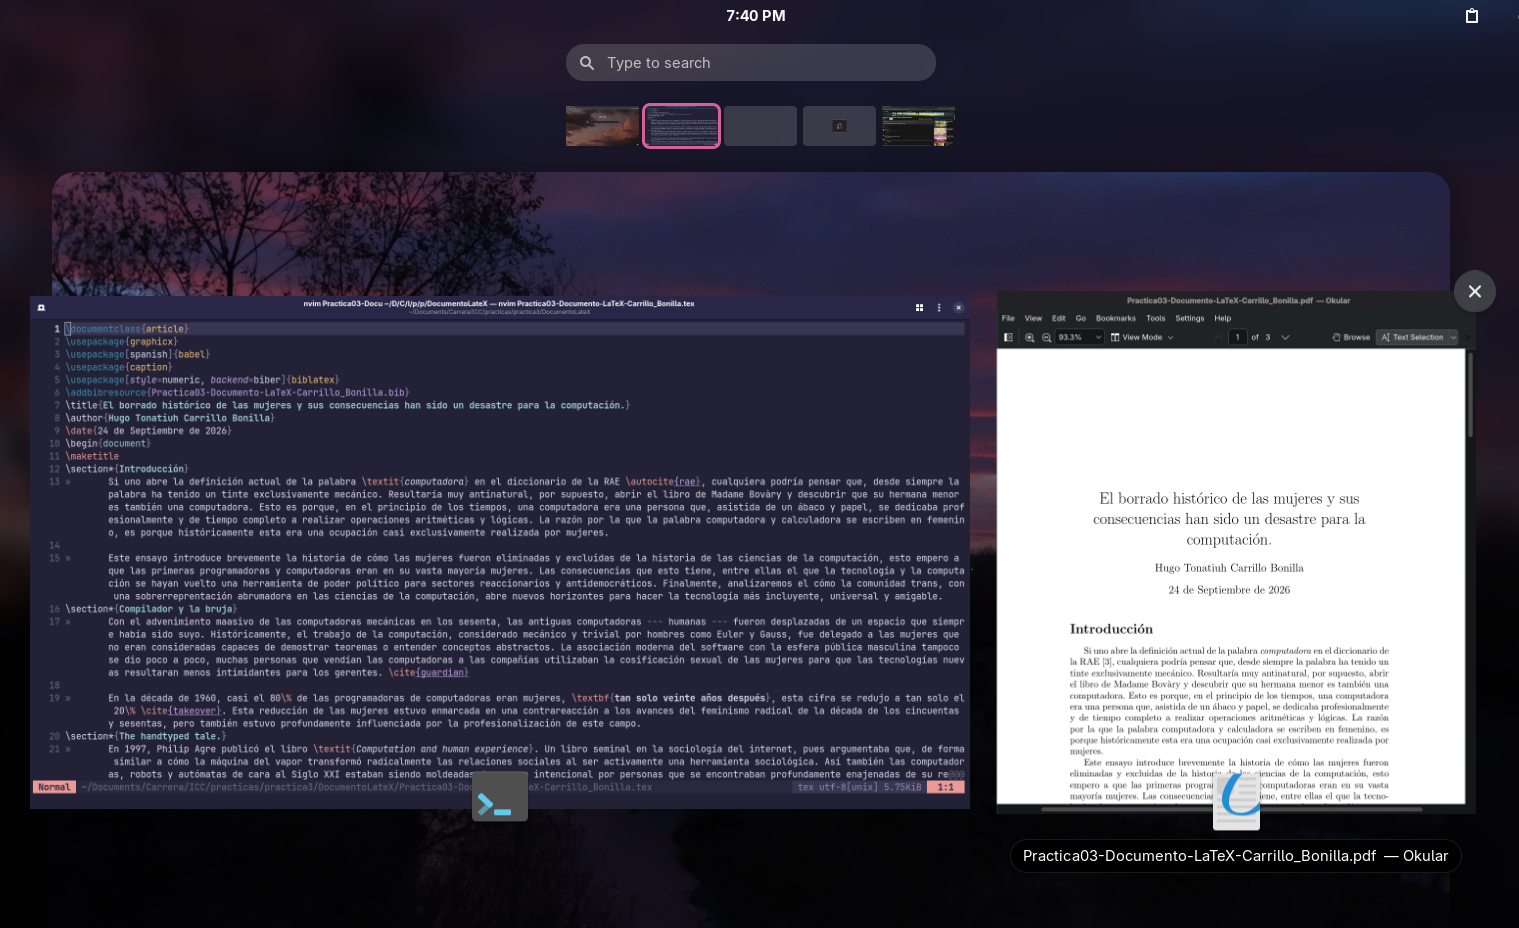
\includegraphics[width=0.5\linewidth]{./images/P1-1.png}
			\end{center}
			Un gran ejemplo de esto fue que aprendí a hacer mi propio archivo \texttt{.bib} realizando esta práctica y esto a su vez me proporcionó aprendizaje sobre cómo funcionan los objetos flotantes en \LaTeX y cómo inicializan los paquetes, ya que al principio mi archivo no compilaba. Para resolver esto usé la siguiente bibliografía:
			\printbibliography[keyword=parte1, title={Referencias Parte 1}, heading=subbibliography]
	\section*{Parte 2: Git.}
		\subsection*{Actividad 2.1: Su primer repositorio.}
			Lamentablemente, yo ya venía desarrollando mis prácticas en un repositorio de \texttt{git}. Afortunadamente, este repositorio era exclusivamente local, por lo que no tuve que deshacerme de remotos ajenos (algo que no tengo ni idea de cómo se hace).
			\begin{center}
				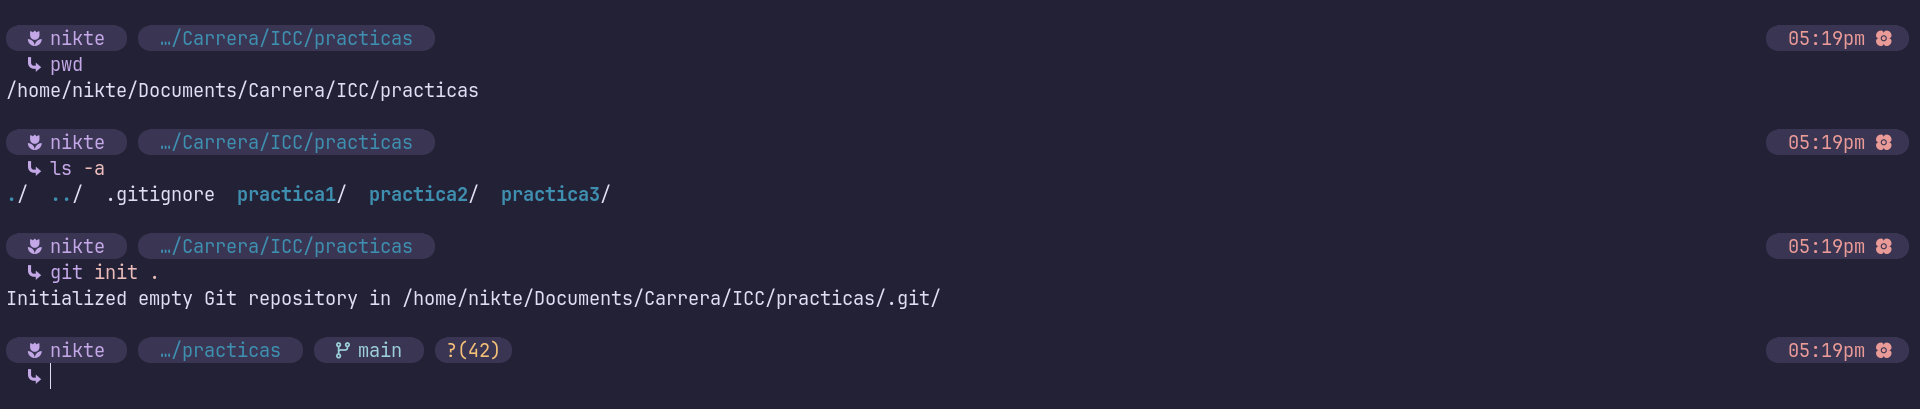
\includegraphics[width=\linewidth]{./images/P2-1-1.png}
			\end{center}
			Markdown permite usar MathJax
			\begin{center}
				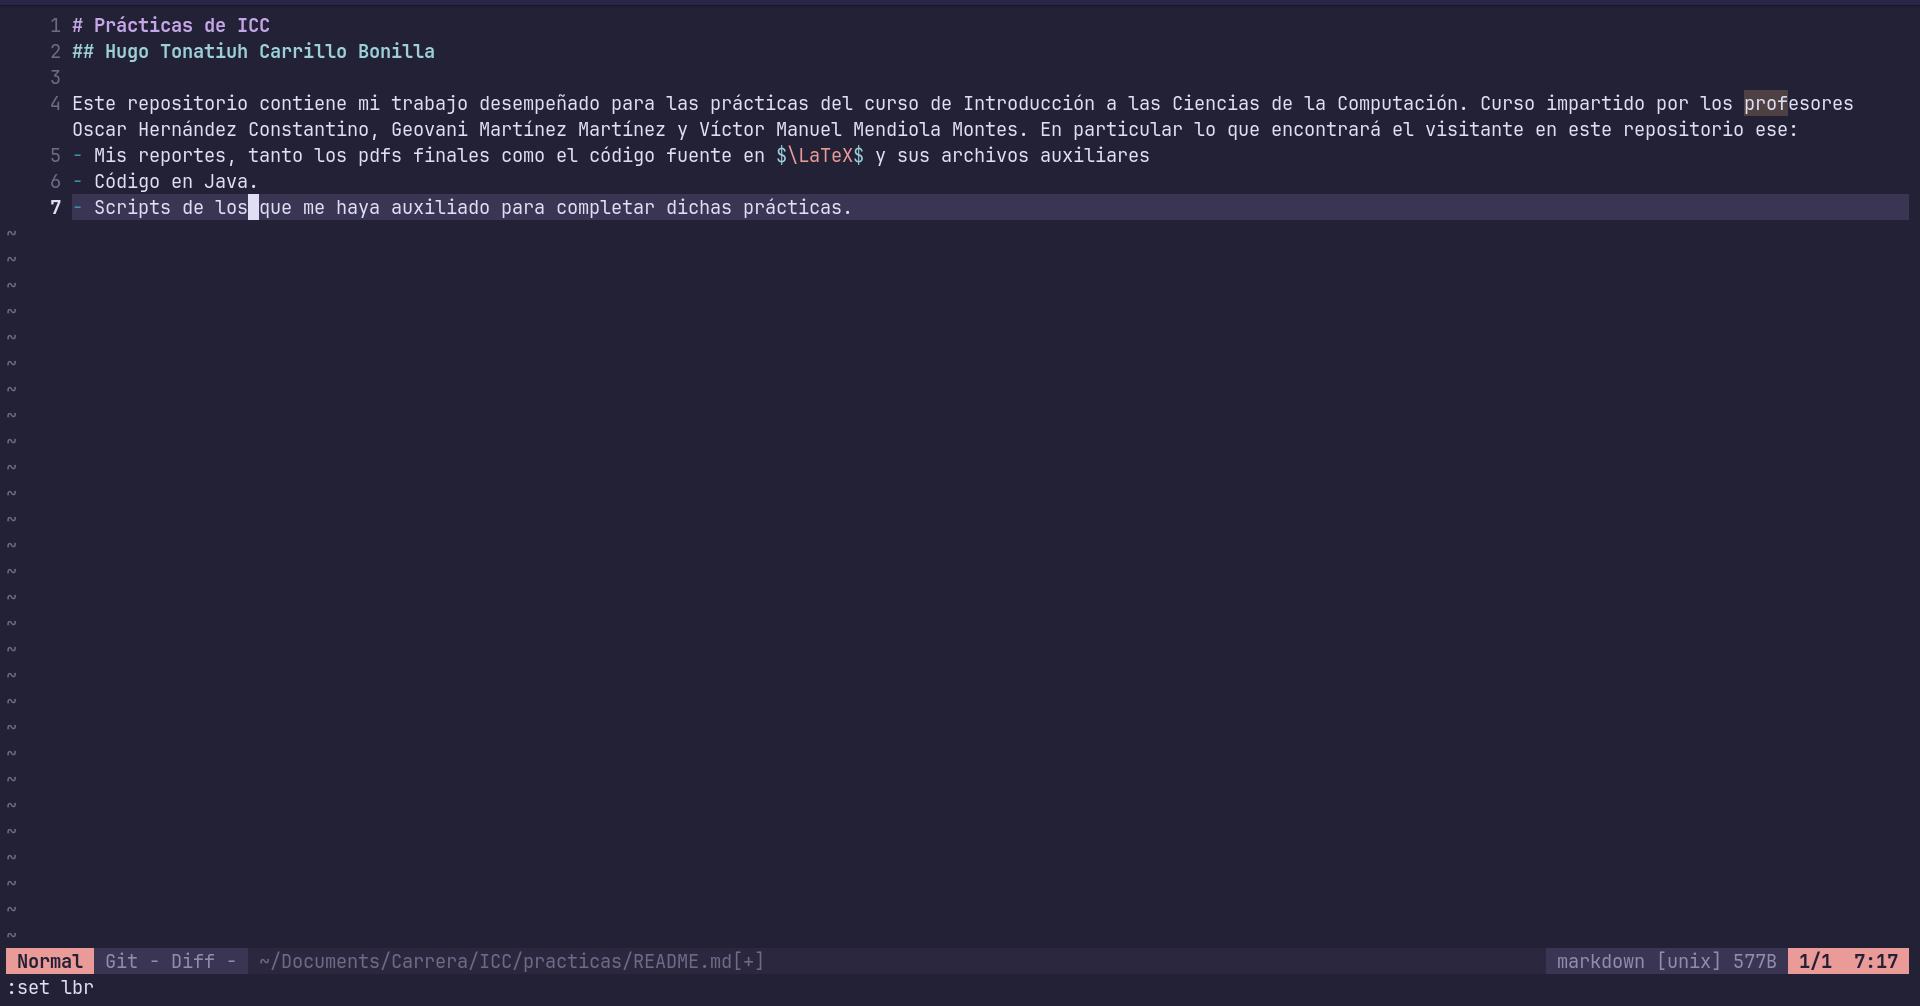
\includegraphics[width=\linewidth]{./images/P2-1-2.png}
			\end{center}
			Una vez que tuve todos mis archivos en orden, hice staging y publiqué mis cambios a mi rama de git.
			\begin{center}
				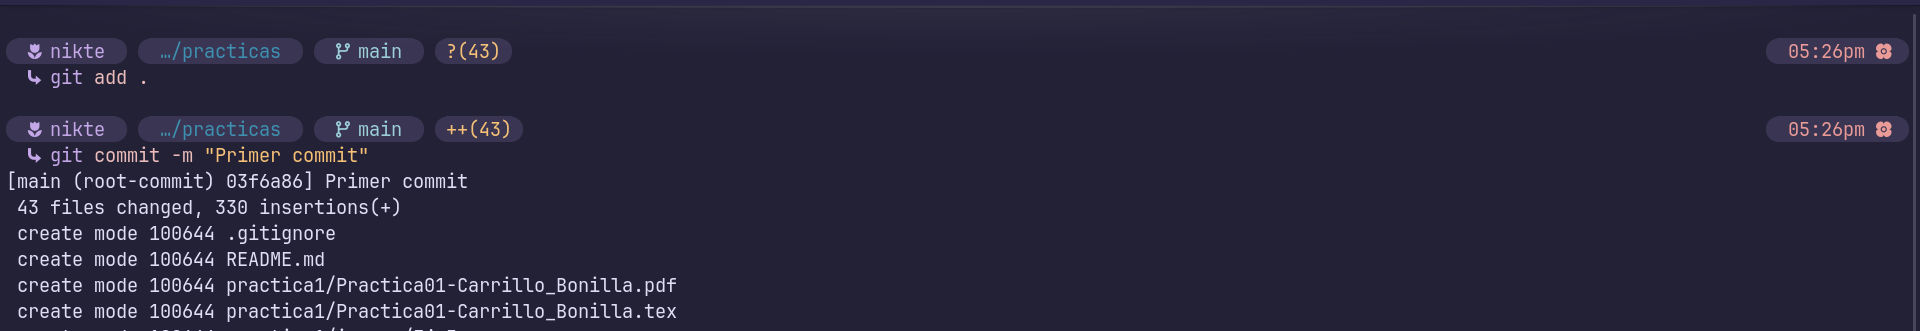
\includegraphics[width=\linewidth]{./images/P2-1-3.png}
			\end{center}
			Creé un repositorio vacío en github y mejor subí todo lo que ya había hecho, vinculándolo a través de \texttt{https}. (Una decisión de la que muy rápido me arrepentiría).
			\begin{center}
				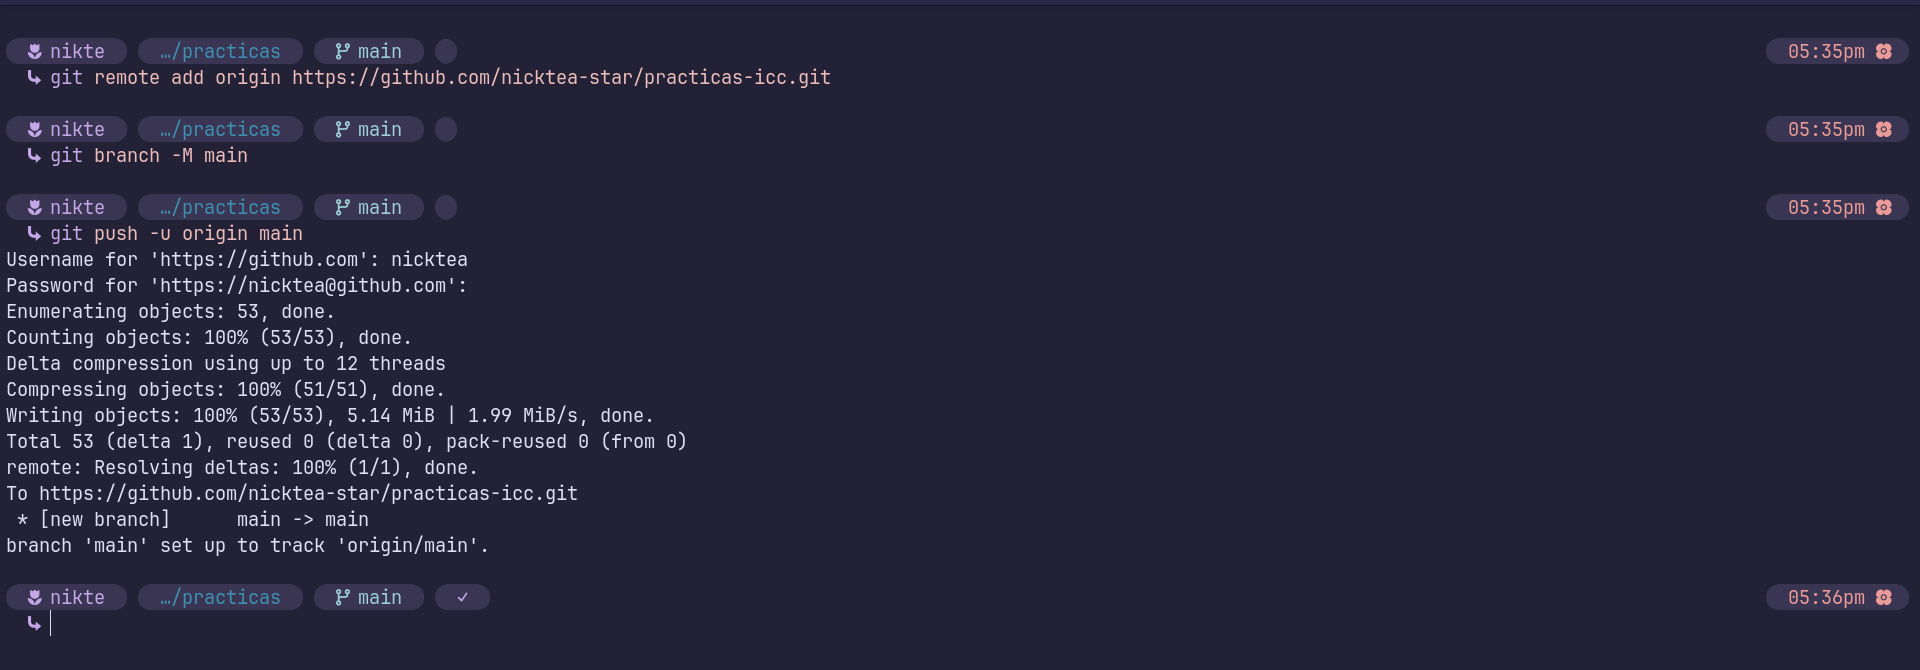
\includegraphics[width=\linewidth]{./images/P2-1-4.png}
			\end{center}
			Evidencia de que pude subir mi repositorio a Github de forma exitosa.
			\begin{center}
				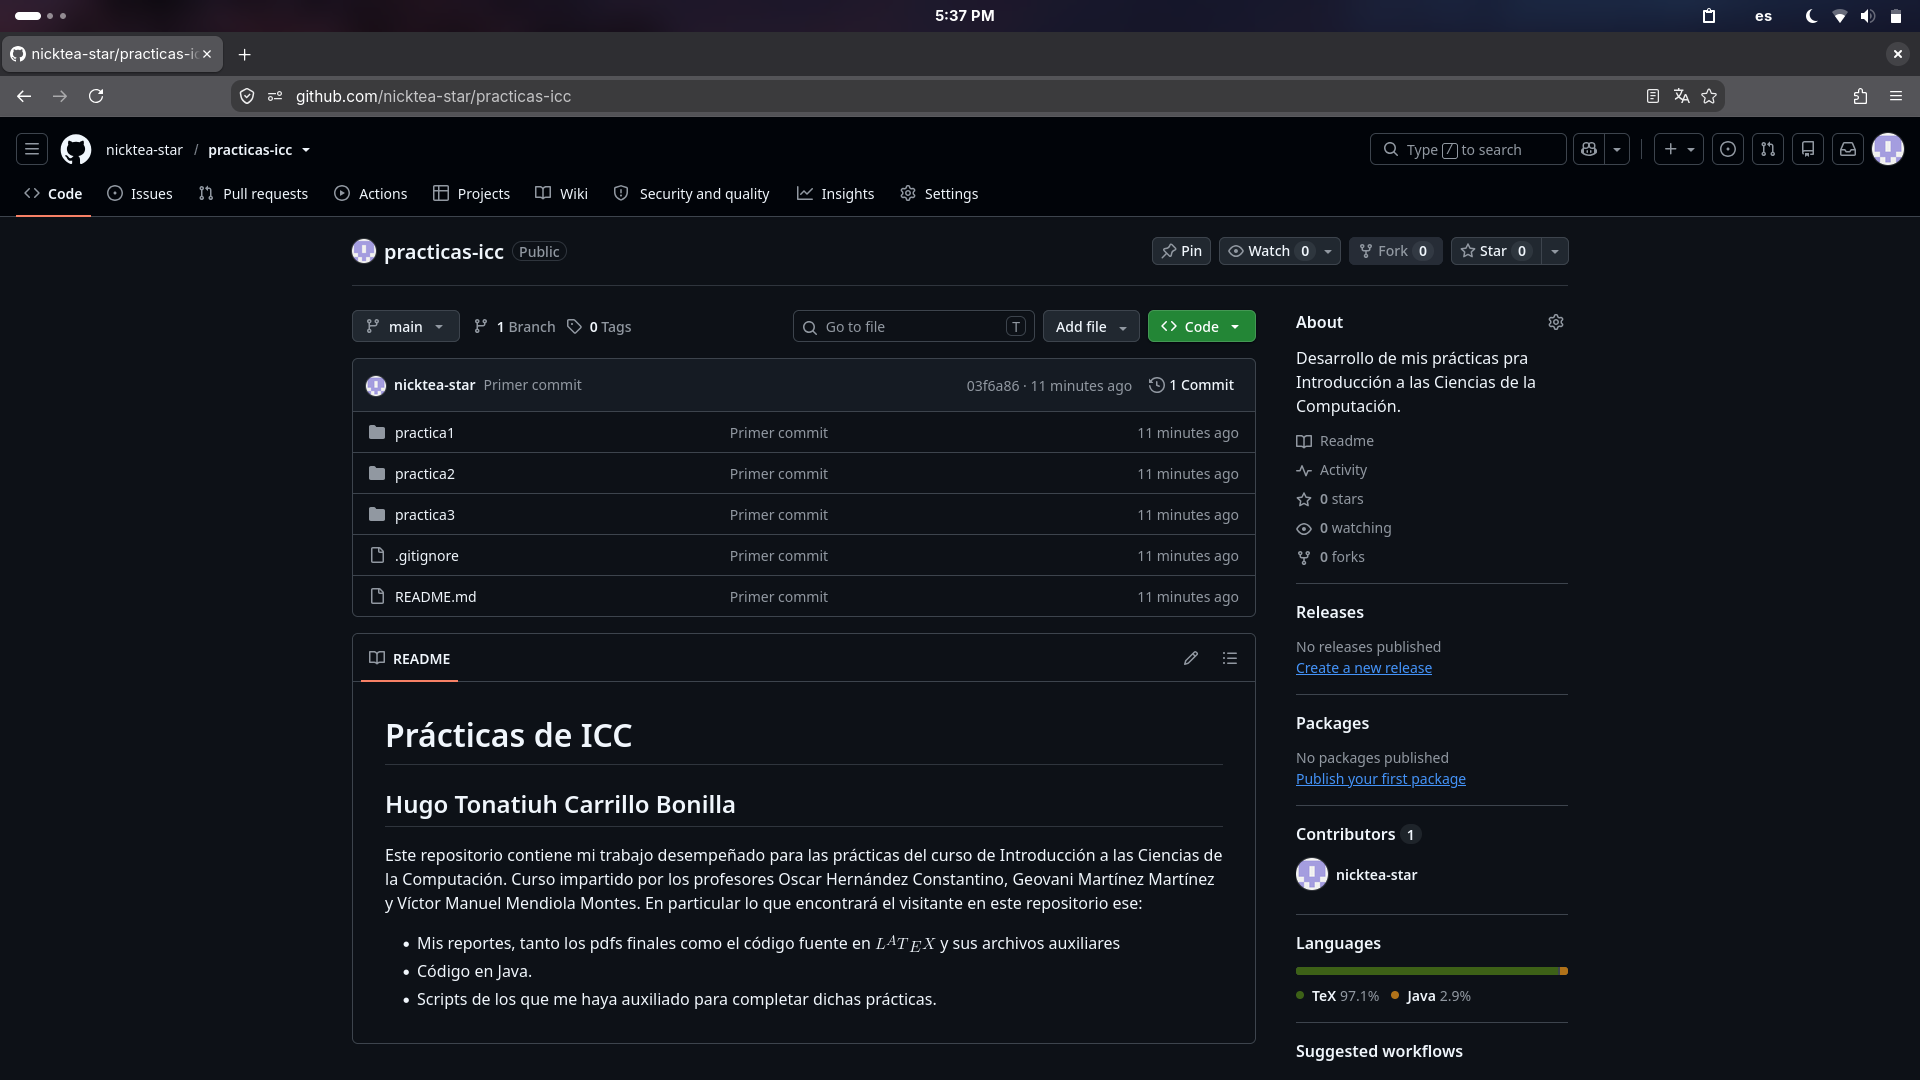
\includegraphics[width=\linewidth]{./images/P2-1-5.png}
			\end{center}
		\subsection*{Actividad 2.2: Guardar su documento de \LaTeX.}
			Como ya tenía un directorio para mi práctica 3 para redactar el documento que actualmente estás leyendo, renombré a los directorios que estaban dentro de mi repositorio.
			\begin{center}
				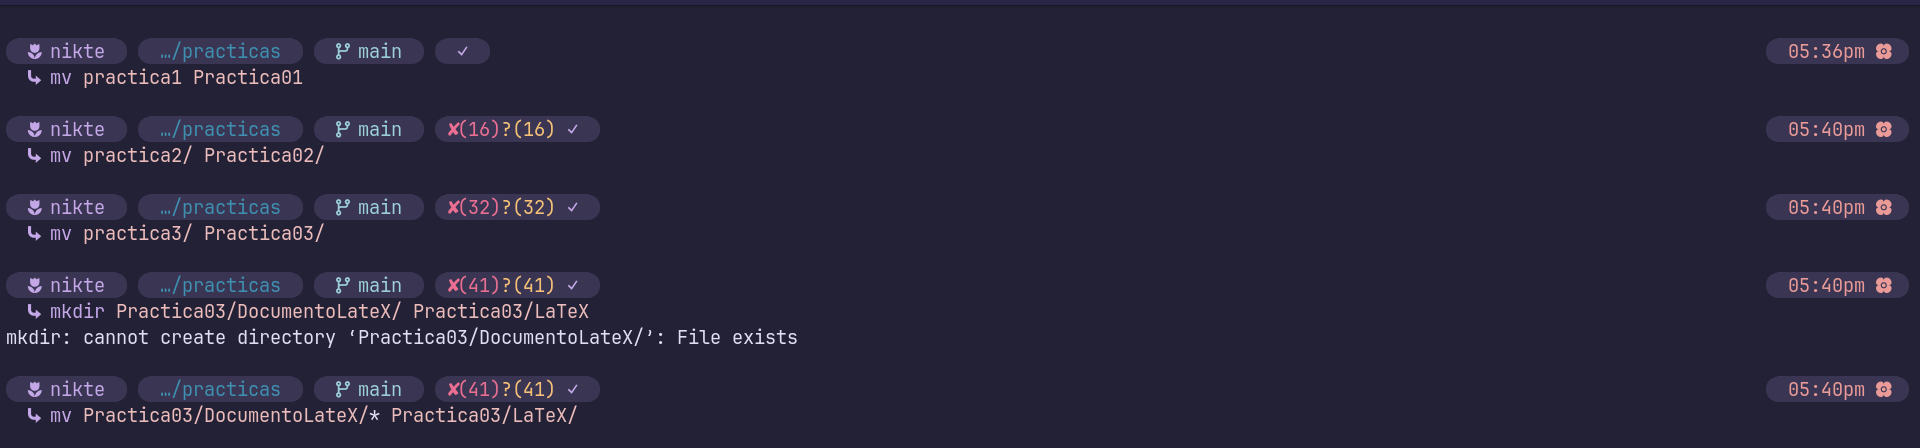
\includegraphics[width=\linewidth]{./images/P2-2-1.png}
			\end{center}
			Por alguna razón, el directorio \texttt{DocumentoLaTeX}, donde tenía originalmente mi archivo de \LaTeX era reacio a renombrarse y después ser borrado.
			\begin{center}
				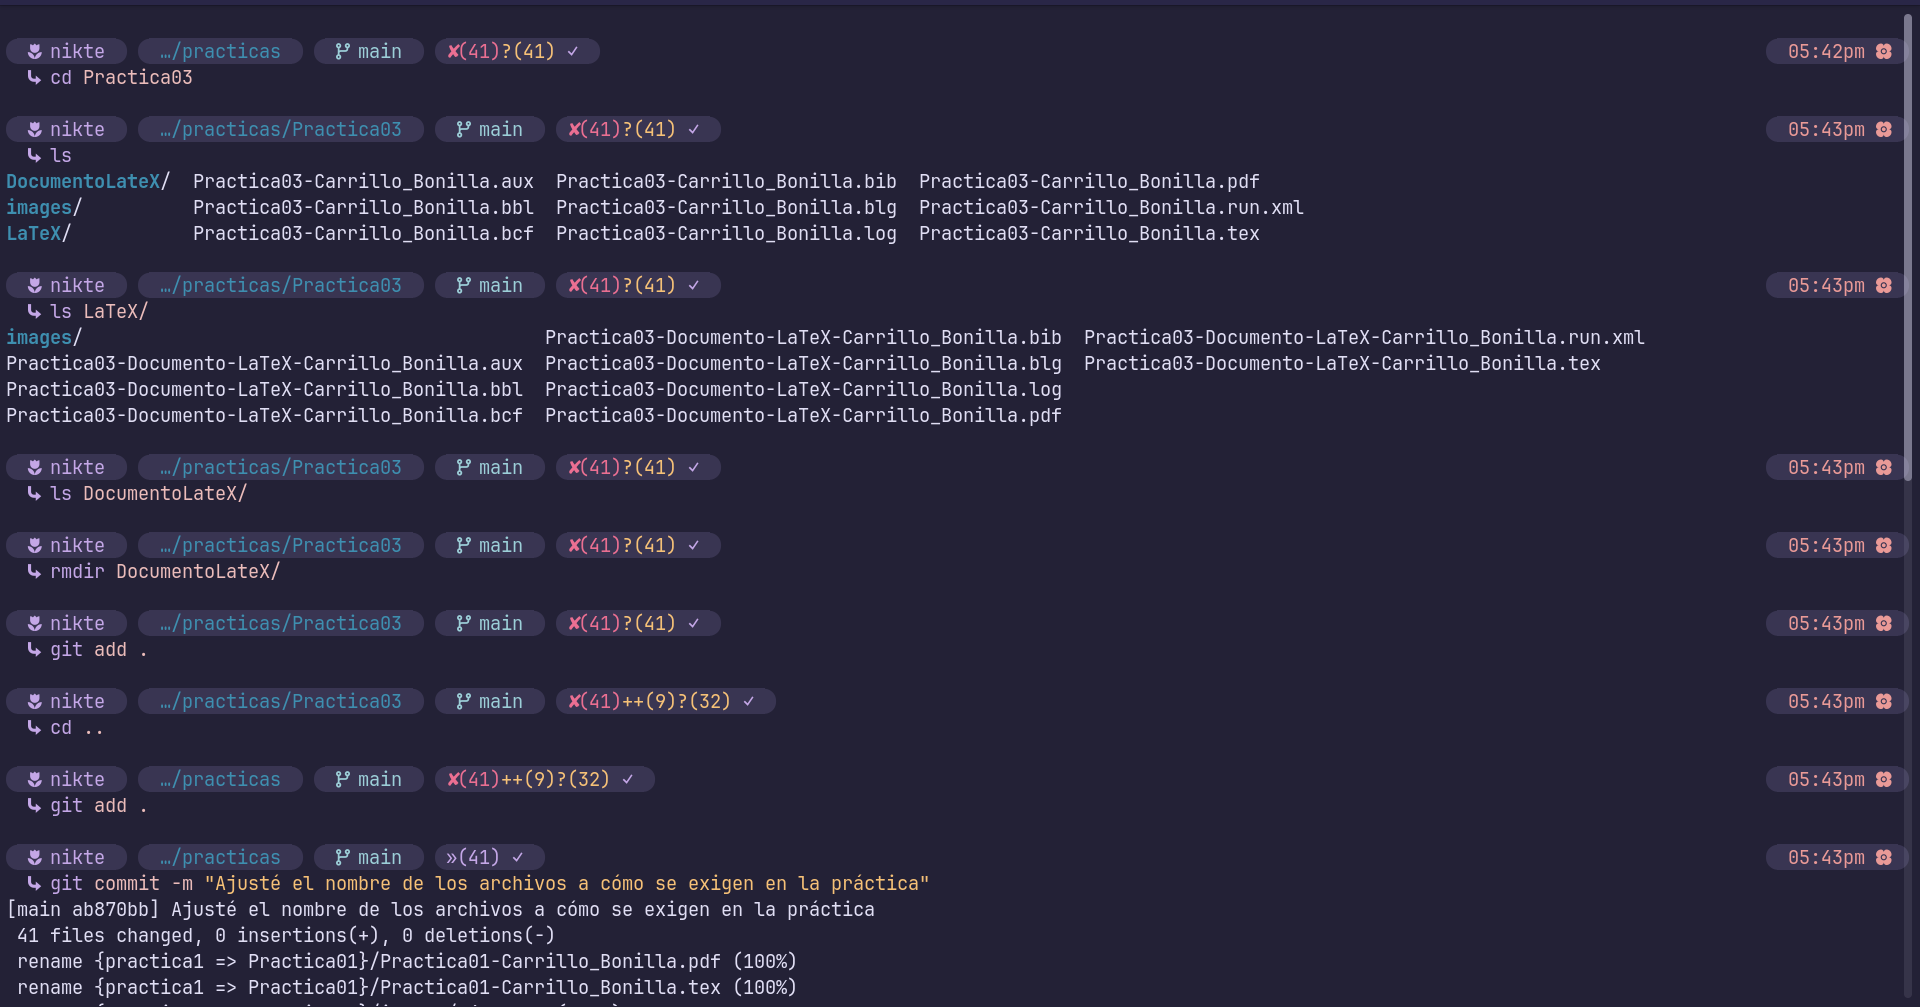
\includegraphics[width=\linewidth]{./images/P2-2-2.png}
			\end{center}
			Para no tener que revalidar mi token (lo generé por un solo día), preferí utilizar \texttt{ssh} y añadir el repositorio git de esa manera. Aprendí a hacer esto en la documentación de Github. \cite{github}
			\begin{center}
				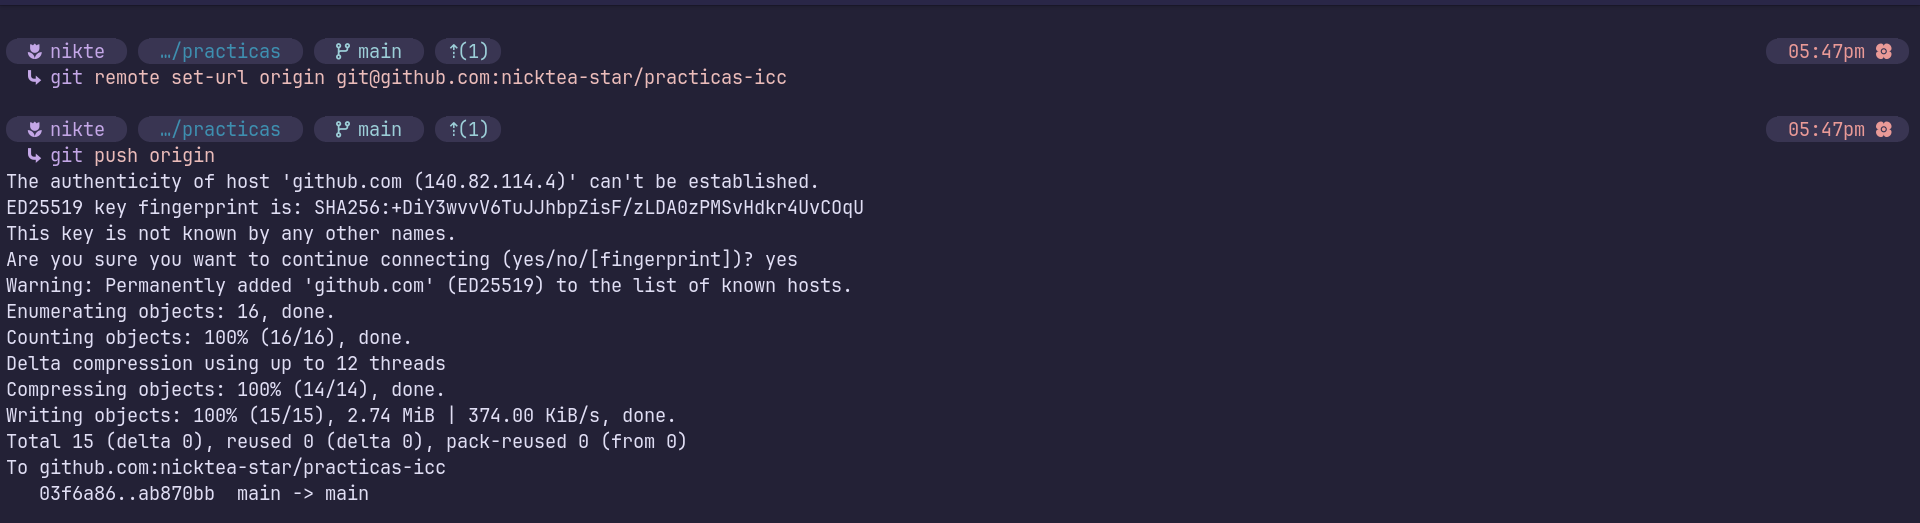
\includegraphics[width=\linewidth]{./images/P2-2-3.png}
			\end{center}
			\begin{center}
				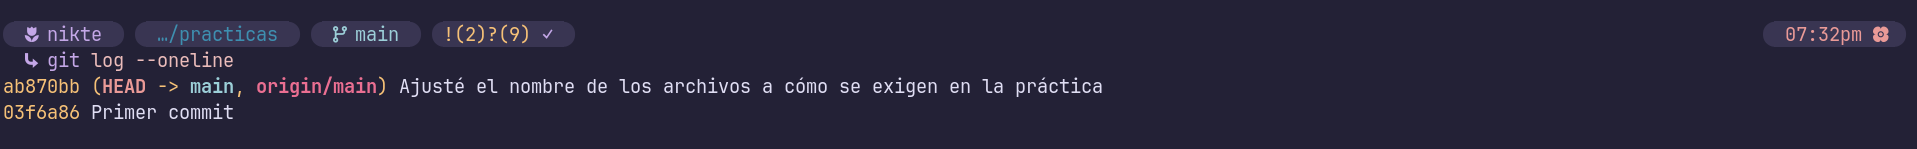
\includegraphics[width=\linewidth]{./images/P2-2-4.png}
			\end{center}
			Sobre la bibliografía, realmente ya sabía hacer todo estoen Git, pero supongo que si tengo que indicar un recurso sería el libro oficial que viene en la página oficial del proyecto \cite{gitbook}.
			\printbibliography[keyword=parte2, title={Referencias Parte 2}, heading=subbibliography]
\end{document}

